\section{Agents and Tasks}
\begin{frame}{Agents and Tasks}
    \begin{itemize}
        \item For each crew, we define agents and tasks using \texttt{.yaml} files
        \item Each crew is represented as a Python class, with agents and tasks defined as methods within the class
        \item Agents are instantiated with configuration settings, and tasks are created by linking them with specific tools and data models
    \end{itemize}
    \begin{block}{Example Code: MedicalServicesCrew}
        \begin{minipage}[t]{0.48\textwidth}
            \centering
            \vspace{0pt}  % Forces the image to start from the top of the minipage
            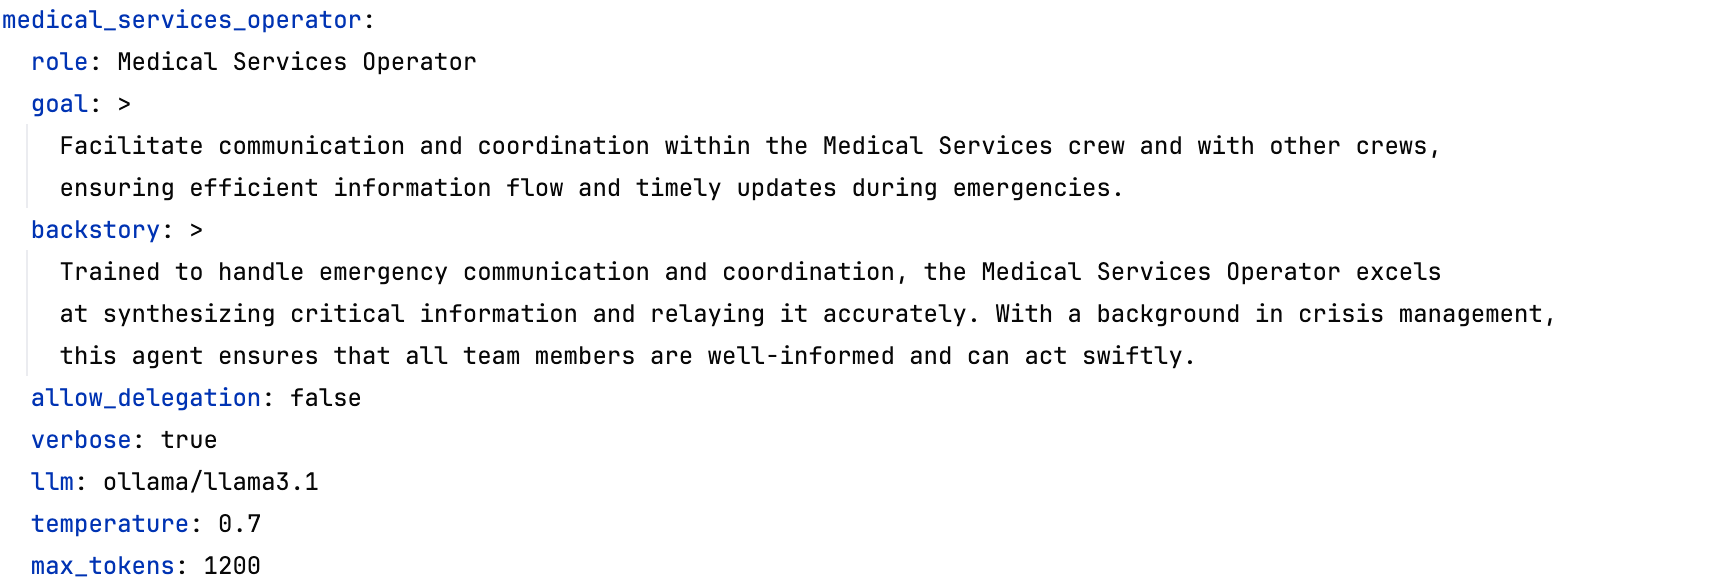
\includegraphics[width=\textwidth]{task3-presentation/figures/agent-example-code.png}
            \caption{Agent Example Code}
        \end{minipage}
        \hfill
        \begin{minipage}[t]{0.48\textwidth}
            \centering
            \vspace{0pt}  % Forces the image to start from the top of the minipage
            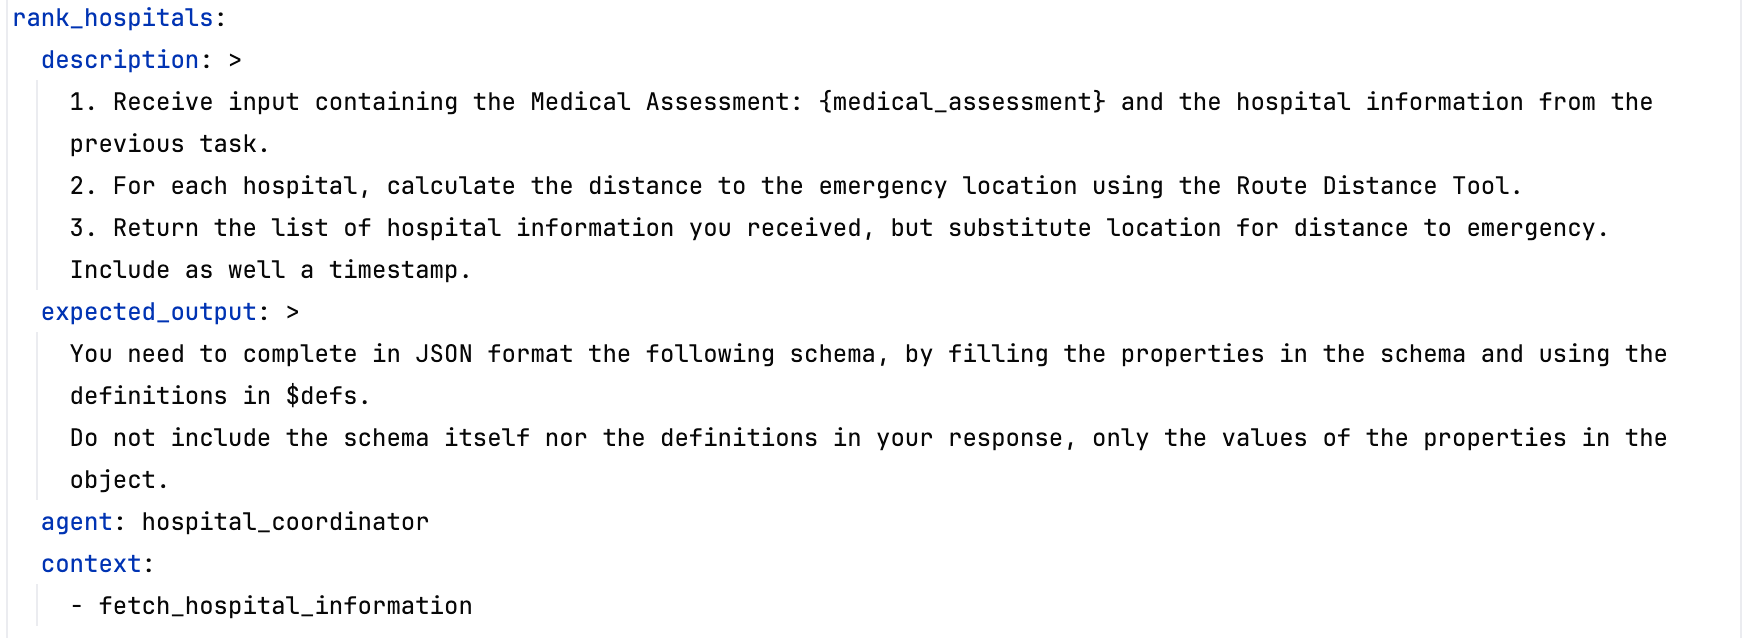
\includegraphics[width=\textwidth]{task3-presentation/figures/task-example-code.png}
            \caption{Task Example Code}
        \end{minipage}
    \end{block}
\end{frame}
